\documentclass[11pt]{article}
\usepackage{amssymb,amsmath,amsthm}
\usepackage{bm, mathrsfs}
\usepackage{graphicx}
\usepackage{geometry}
\usepackage{textcomp}
\usepackage{hyperref}
\usepackage{ragged2e}
\usepackage{float}
\graphicspath{ {./images/} }
\newtheorem{remark}{Remarque}
\newcommand{\bx}{\bm{x}}

\title{ISC3, Fall 2022(A22)\\
Computer works report TP 1, 19/09/2022}
\author{Wenlong CHEN}
\date{October 5, 2022}

\begin{document}
    \maketitle
    \section*{Excercise1}
    Consider the function f defined in $[-1,1]$by
    $$
    f(x)=\frac{1}{1+25x^2}
    $$
    From f, generate a dataset made of the couples $(xi, yi)_{i=0,\ldots,n}$ defined by $x_i=-1+\frac{2i}{n}$,$y_i=f(x_i)$ We are looking for the interpolation polynomial $p_n$ of degree less than or equal to n such $p_n(x_i) = f(x_i)$. For that we will use the Lagrange polynomials $L_i(x)$ seen in the course, then $p_n(x)$ will be written
    $$
    p_n(x)=\sum_{i=0}^ny_iL_i(x)
    $$
    with
     $$
    L_i(x) = \prod_{k=0,k\neq i}\frac{x-x_k}{x_i-x_k}
    $$
    a) Pick up the script in the chapter that implements the Lagrange polynomials$L_i(x)$,then write a Scilab function
    \\$function y = poly\_interp(x, xi, yi)$\\
    ......\\
    with two entry vectors $x_i$ and $y_i$ that contain the $x_i$, $y_i$ and returns the interpolation function value y at point x.\\
    \\
    Solution:\\

    
    \begin{verbatim}
        function y=LagrangePol(x,xj,i)
            numer = ones(x)
            denom=1.0;
            l=length(xj)
            setindex=setdiff(1:l,i)
            for j=setindex
                numer=numer.*(x-xj(j))
                denom=denom.*(xj(i)-xj(j))
            end
            y=numer/denom
        endfunction

        function y=polinterpolation(x,xi,yi)
            y=0*x;
            l=length(xi)
            for i=1:l
                y=y+yj(i) *LagrangePol(x,xi,i)
            end
        endfunction
    \end{verbatim}
    b) Show graphically the lack of convergence of $p_n$ to f using n between 2 and 20(Runge instability phenomenon). Superpose the the respective plots on the same graphics.\\
    
    Solution:
    \begin{figure}[H]
        \centering
        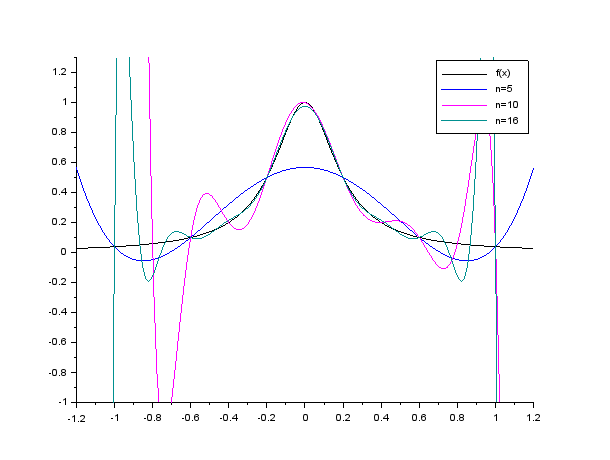
\includegraphics[scale=0.38]{inter}
        \caption{L'image de l'interpolation}
    \end{figure}
    Code pour cette question :
    \begin{verbatim}
        x1=linspace(-1.5,1.5,200)
        plot2d(x1,f(x1),rect=[-1.2,-0.3.2,1.3],style=1)

        function plot_inter(n0,col)
            xi=zeros(n0)
            for z=1:n0
                xi(z)= -1+2*z./n0
            end
            //plot(xi,f(xi),'o')
            plot2d(x1,polinterpolation(x1, xi,f(xi)),rect=[-1.2,-0.3.2,1.3],style=col)
        endfunction

        plot_inter(5,2)
        plot_inter(10,7)
        plot_interpp(15,16)
        legend("f(x)", "n=2","n=7","n=16");
    \end{verbatim}


    c) Use the Scilab pre-implemented splin() and interp functions to interpolate the date by means of cubic splines $s_n(x)$. Again, make n vary between 2 and 20. Plot the interpolated function, and compare with polynomial interpolation.\\
    
    Solution:
    \begin{figure}[H]
        \centering
        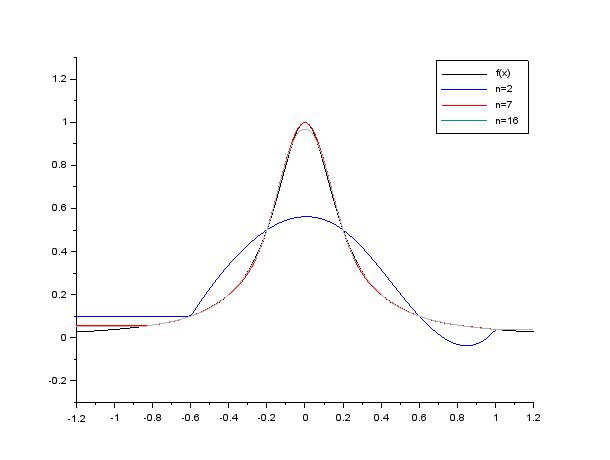
\includegraphics[scale=0.4]{spli}
        \caption{L'image de cubic spline}
    \end{figure}
    Code pour cette question :
    \begin{verbatim}
        function plot_spline(n0,col)
            xi=zeros(n0)
            for z=1:n0
                xi(z)= -1+2*z./n0
            end
            //plot(xi,f(xi),'o')
            d=splin(xi,f(xi))
            yyi=interp(x1,xi,f(xi),d)
            plot2d(x1,yyi,style=3,rect=[-1.2,-0.3,1.2,1.3],style=col)
        endfunction
        plot_spline(5,2)
        plot_spline(10,5)
        plot_spline(15,16)
        legend("f(x)", "n=2","n=7","n=16");
    \end{verbatim}




    \section*{Excercise2}
    Consider$ x_1 = 1$, $x_2 = 2$ and $x_3 = 3$, the cubic polynomial $p_1(x)$ defined in $[x_1,x_2]$ by
    \[p_1(x)=a_0+a_1x+a_2x^2+a_3x^3\]
    And the cubic polynomial $p_2(x)$ defined in $[x_2,x_3]$ by
    \[p_2(x)=b_0+b_1x+b_2x^2+b_3x^3\]
    We want to find $(a_0,a_1,a_2,a_3,b_0,b_1,b_2,b_3)$ such that the following conditions are satisfied:
    \begin{align*}
        &p_1(x_1)=1,\\
        &p_1(x_2)=p_2(x_2)=2,\\
        &p_2(x_3)=0,\\
        &p_1'(x_2)=p_2'(x_2),\\
        &p_1''(x_2)=p_2''(x_2),\\
        &p_1''(x_2)=p_2''(x_2)=x\\
    \end{align*}
    \raggedright
    We have 8 equations for 8 unknowns. Write the linear system of unknown vector $(a_0,a_1,a_2,a_3,b_0,b_1,b_2,b_3$). Solve the linear system, then plot the resulting spline in the interval $[x_1,x_3]$. Check that the spline is a regular function in the interval (especially at $x_2$).\\
    Solution:\\
    Sur la base de la définition de l'interpolation par spline cubique, nous pouvons obtenir la matrice de coefficients suivante:
    $$
    \begin{bmatrix}
        1&1&1&1&0&0&0&0\\
        1&2&4&8&0&0&0&0\\
        0&0&0&0&1&2&4&8\\
        0&0&0&0&1&3&9&27\\
        0&1&4&12&0&-1&-4&-12\\
        0&0&2&12&0&0&-2&-12\\
        0&0&2&6&0&0&0&0\\
        0&0&0&0&0&0&2&18
    \end{bmatrix}
    *
    \begin{bmatrix}
        a_0\\a_1\\a_2\\a_3\\b_0\\b_1\\b_2\\b_3
    \end{bmatrix}
    =
    \begin{bmatrix}
        1\\2\\2\\0\\0\\0\\x\\x
    \end{bmatrix}
    $$
    En résolvant l'équation et en dessinant l'image de la fonction, on obtient
    \begin{figure}[H]
        \centering
        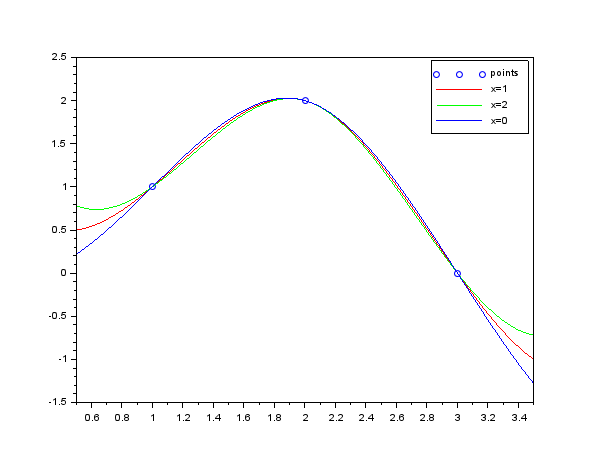
\includegraphics[width=0.8\textwidth,height=0.5\textwidth]{spline}
        \caption{L'image de cubic spline}
    \end{figure}
    Comme x varie, la fonction s'incurve différemment aux deux extrémités,il est le plus naturel à x = 0.\\
    ~\\~\\
    Code pour cette question:
    \begin{verbatim}
        xi=1

        A=[1,1,1,1,0,0,0,0;
        1,2,4,8,0,0,0,0;
        0,0,0,0,1,2,4,8;
        0,0,0,0,1,3,9,27;
        0,1,4,12,0,-1,-4,-12;
        0,0,2,12,0,0,-2,-12;
        0,0,2,6,0,0,0,0;
        0,0,0,0,0,0,2,18;]

        b=[1;2;2;0;0;0;xi;xi]
        coef=A\b

        function f=functionA(coef,x)
            xA=x(x>=0.5&x<=2)
            f(find(x>=0.5&x<=2))= coef(1)+coef(2)*xA+coef(3)*xA^2+coef(4)*xA^3
            xB=x(x>2&x<=3.5)
            f(find(x>2&x<=3.5))= coef(5)+coef(6)*xB+coef(7)*xB^2+coef(8)*xB^3
        endfunction
        x=linspace(0.5,3.5,100)
        x0=[1,2,3]
        y0=[1,2,0]
        plot(x0,y0,'o')

        plot(x,functionA(coef,x),'r')
        xi=2
        b=[1;2;2;0;0;0;xi;xi]
        coef=A\b
        plot(x,functionA(coef,x),'g')
        xi=0
        b=[1;2;2;0;0;0;xi;xi]
        coef=A\b
        plot(x,functionA(coef,x),'b')
        legend("points","x=1", "x=2","x=0");
    \end{verbatim}

    \section*{Résumé}
    Comme nous pouvons le voir, ce n'est pas le cas que plus le nombre de polynômes est élevé, meilleur est le résultat ; l'erreur d'un polynôme plus élevé au bord de l'intervalle de la fonction peut être significative, c'est le phénomène de Longe pour les polynômes supérieurs.
    Et ce problème est bien évité par l'utilisation d'une fonction spline cubique
\end{document}